\chapter{Предварительные сведения}

\section{Самоподобные множества и дендриты}

\subsection{Самоподобные множества}

Базовым понятием в теории самоподобных множеств является понятие аттрактора системы сжимающих отображений.
%Аттрактор мы также называем самоподобным множеством.
%Самоподобным множеством мы называем множество, являющееся объединением своих уменьшеных копий.

\begin{restatethis}{definition}{dfn:sss}%[J. Hutchinson (1981), см. {\cite{Hut1981}}]
 %\label{dfn:sss}
{\em (J. Hutchinson (1981), см. {\cite{Hut1981}})} 
Пусть $\eS=\{S_1, S_2, \ldots, S_m\}$ ---  система (иньективных) сжимающих отображений полного метрического пространства $(X, d)$.
Непустое компактное множество $K\IN X$ называется аттрактором системы $\eS$, если 
$$K = \bigcup \limits_{i=1}^m S_i (K).$$
Мы также называем множество $K$ самоподобным (инвариантным) относительно системы $\eS$.
\end{restatethis} 
\begin{definition} Переписать
Для системы $\eS=\{S_1,\ldots,S_m\}$ сжимающих подобий в $\rr^n$  равенством $T(A)=\bigcup\limits_{i=1}^m S_i(A)$ задаётся  оператор Хатчинсона $T$ на пространстве $C(\rr^n)$ непустых компактов в $\rr^n$ .
\end{definition}

Cогласно Теореме Хатчинсона, аттрактор $K$ существует и единственен для $\eS$, а для любого компактного множества $A\IN X$ последовательность $T^n (A)$ сходится к $K$.
Это действительно так, ведь если $C(\rr^n)$ --- полное метрическое гиперпространство непустых компактов из $\rr^n$ с метрикой Хаусдорфа, то оператор Хатчинсона $T$ системы $\eS$ в этом пространстве является сжимающим отображением, а значит $T$ имеет в нём единственную неподвижную точку $K=T(K)$, которой и является аттрактор системы $\eS$.\\

{\em Подобием} мы называем преобразование евклидова пространства, при котором для любых двух точек $A, B$ и их образов $A',B'$ имеет место соотношение $|A'B'|=q\cdot |AB|$ при некотором фиксированном $q\neq 0$, называемым {\em коэффициентом подобия}.
Тогда подобие можно представить как суперпозицию гомотетии, параллельного переноса и ортогонального преобразования.
На протяжении всей главы предполагается, что отображения $S_i\in \eS$ являются сжимающими подобиями, а множество $X$ --- это $\mathbb{R}^2$.
Поэтому мы будем использовать комплексные обозначения для точки на плоскости, поэтому каждое подобие может быть записано как $S_j(z)=q_j e^{i\al_j}(z-z_j)+z_j$, где $q_j=\Lip S_j$ и $z_j=\fix(S_j)$.

Как уже говорилось выше, коэффициент $q_j=\Lip S_j$ мы называем {\em коэффициентом подобия} отображения $S_j$.
Для системы $\eS=\{S_1, S_2, \ldots, S_m\}$ обозначим $q_{min}=\min\{q_j,\ j=1,\ldots,m\}$ и $q_{max}=\max\{q_j,\ j=1,\ldots,m\}$ --- минимальный и максимальный коэффициенты подобия отображений системы $\eS$.\\

Важным и полезным инструментом при описании и изучении самоподобного множества является индексная параметризация точек и копий самоподобного множества.
Пусть дана система $\eS=\{S_1, S_2, \ldots, S_m\}$.
Тогда $I=\{1,2,\ldots,m\}$ --- это {\em множество индексов} системы $\eS$, в то время как $\ia=\bigcup\limits_{n=1}^\8 I^n$ мы называем {\em множеством всех мультииндексов конечной длины} $\bj=j_1 j_2 \ldots j_n$.
Длина $n$ мультииндекса $\bj=j_1...j_n$ обозначается как $|\bj|$, а $\bi\bj$ обозначает конкатенацию соответствующих мультииндексов. 
Мы говорим, что $\bi\sqsubset\bj$, если  $\bj=\bi\bl$ с некоторым $\bl\in\ia$, то есть слово $\bi$ является началом слова $\bj$. 
Если $\bi\not\sqsubset\bj$ и $\bj\not\sqsubset\bi$, то $\bi$ и $\bj$ называем {\em несравнимыми}.

Для мультииндекса $\bj\in\ia$ мы пишем $S_\bj=S_{j_1j_2\ldots j_n}=S_{j_1}S_{j_2}\ldots S_{j_n}$ и для аттрактора $K=K(\eS)$ мы обозначим $S_\bj(K)$ как $K_\bj$ и будем называть $K_\bj$ {\em копией степени $n$} самоподобного множества $K$.
Тогда если $\bi\sqsubset\bj$, то $K_\bj\IN K_\bi$.\\

Вместе с системой $\eS$ мы можем рассматривать её $n$-ное измельчение $\eS^{(n)}=\{S_\bj, \bj\in I^n\}$, оператор Хатчинсона которой равен $T^n$.
Мы также обозначим через $G_\eS=\{S_\bj, \bj\in\ia\}$ полугруппу, порожденную системой $\eS$. 

Обозначим $I^{\8}=\{{\bma}=\al_1\al_2\ldots\ |\ \al_i\in I\}$ как {\em индексное пространство} и мультииндекс бесконечной длины $\bma\in I^{\8}$ назовём {\em строкой}.
Тогда пусть $\pi:I^{\8}\rightarrow K$ --- так называемое {\em индексное отображение}, переводящее строку $\bma\in I^{\8}$ в точку $x=\pi(\bma)=\bigcap\limits_{n=1}^\8 K_{\al_1\ldots\al_n}$.\\
Если $\pi(\bma)=x$, то $\bma$ называем {\em адресом} точки $x$. 
Для каждого адреса $\bma$ точки $x\in K$, точка $x_n=S_{\al_1...\al_n}^{-1}(x)$ называется $n$-м предшественником точки $x$, а последовательность $x_1, x_2,...$ называется последовательностью предшественников точки $x$.


\subsection{Размерность и связность самоподобного множества}

В теории самоподобных множеств часто возникает вопрос о вычислении их фрактальной размерности, например размерности Хаусдорфа.
В случае самоподобных множеств мы можем воспользоваться оценкой размерности Хаусдорфа $\dim_H(K)\leq s$, где $s$ --- {\em размерность подобия} системы $\eS$.
Это значение $s$ является решением уравнения Морана $q_1^s+\ldots+q_m^s=1$.

Такая оценка размерности становится равенством $\dim_H(K)=s$, если копии ${K_i, i\in I}$ самоподобного множества $K$ пересекаются друг с другом <<не слишком сильно>>, или, говоря более формально, если система $\eS$ удовлетворяет {\em условию открытого множества}. 

\begin{definition}[J. Hutchinson (1981), см. {\cite{Hut1981}}]\label{dfn:osc}
Будем говорить, что система $\eS=\{S_1,\ldots,S_m\}$ удовлетворяет {\em условию открытого множества} (OSC), если существует непустое открытое множество $O \IN X$ такое, что
\begin{enumerate}[nolistsep]
\item[(1)] $S_i(O)\cap S_j(O)=\0$ для любых различных $S_i,S_j\in\eS$;
\item[(2)] $S_i(O)\IN O$ для любого $S_i\in\eS$.
\end{enumerate}
%что множества из $\{S_i(O): i=1, \ldots, m\}$ попарно непересекаются и все содержатся в $O$.
\end{definition}

Тогда, если система сжимающих подобий $\eS$ удовлетворяет условию открытого множества, то хаусдорфова размерность аттрактора этой системы равна его размерности подобия $s$ (см. \cite{Hut1981, Falconer2004}).

Структура пересечений копий самоподобного множества связана не только с размерностью Хаусдорфа, но ещё и влияет на связность самоподобного множества.
Самоподобное множество может быть связным, несвязным и даже вполне несвязным, и для проверки самоподобного множества на связность мы можем воспользоваться критерием связности М. Хаты \cite[Theorem 4.6]{Hata1985}.
Однако нам удобнее и нагляднее будет использовать интерпретацию критерия связности, для которой нужно построить простой граф пересечений.

\begin{definition}
Обозначим как $\tilde{\Gamma}(\eS)$ граф, вершинам которого соответствуют копии $\{S_i(K):\; S_i\in \eS\}$, а пара вершин $S_i(K),\ S_j(K)$ соединена ребром, если $S_i(K)\cap S_j(K)\neq\0$.
Назовём такой граф {\em простым графом пересечений} для $K(\eS)$.
\end{definition}

\begin{theorem}
Аттрактор $K(\eS)$ системы $\eS$ связен тогда и только тогда, когда его простой граф пересечений $\tilde{\Gamma}(\eS)$ связен.
Тогда аттрактор $K(\eS)$ локально связн и линейно связен.
\end{theorem}

Как видно на следующем рисунке, треугольник Серпинского связен, поскольку его простой граф пересечений связен.

\begin{figure}[h!]
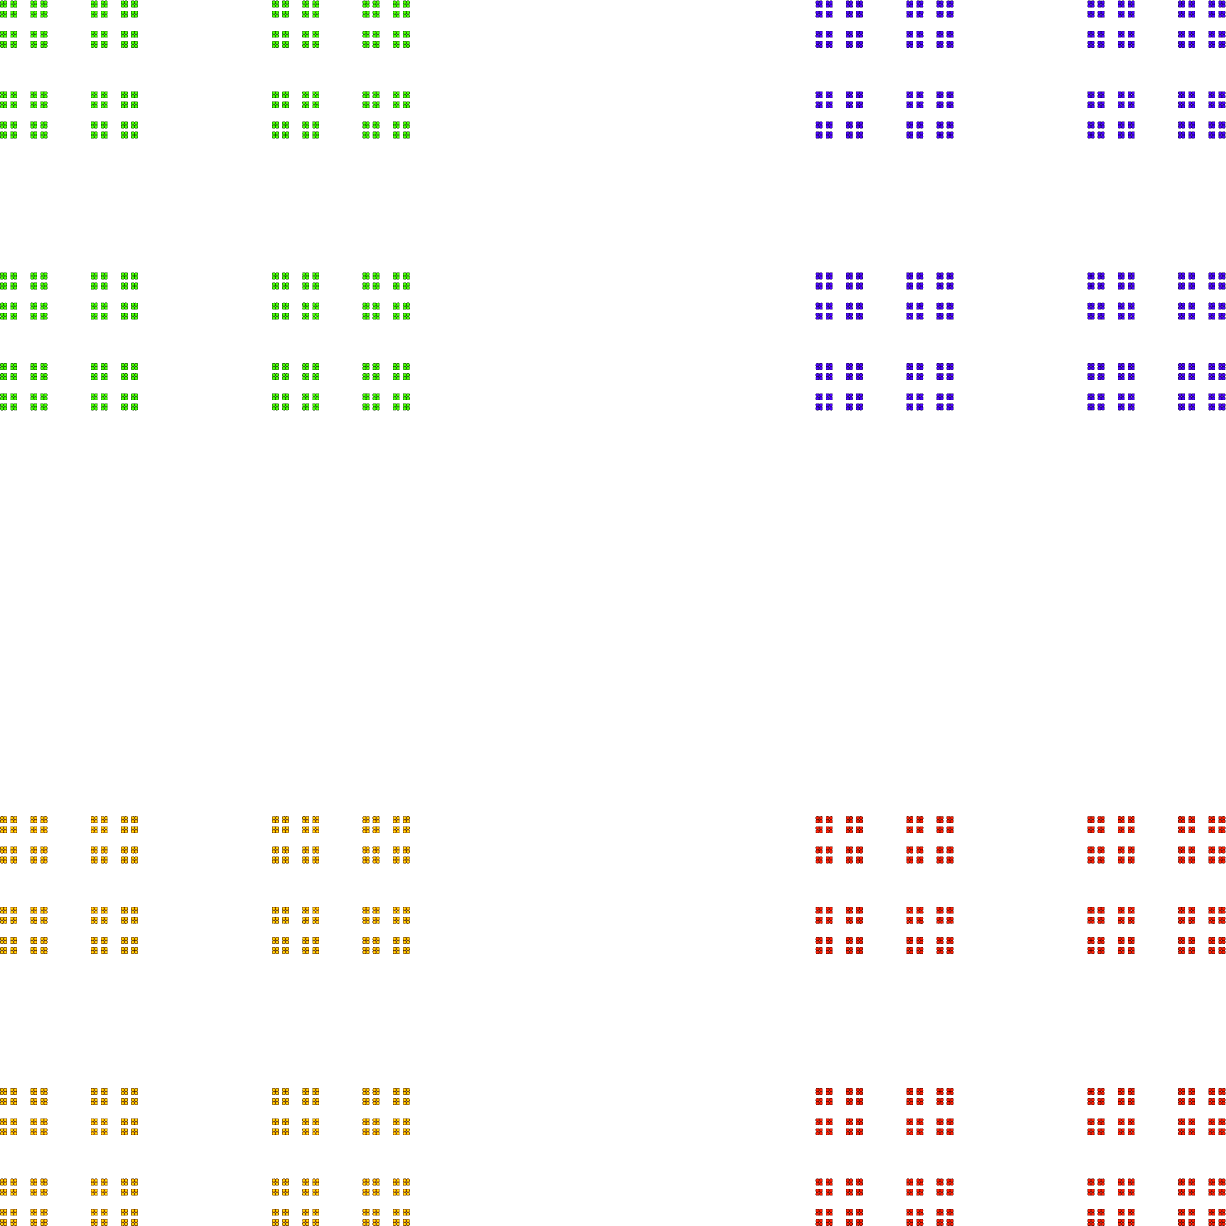
\includegraphics[width=0.3\textwidth]{CS.png}
\hfill
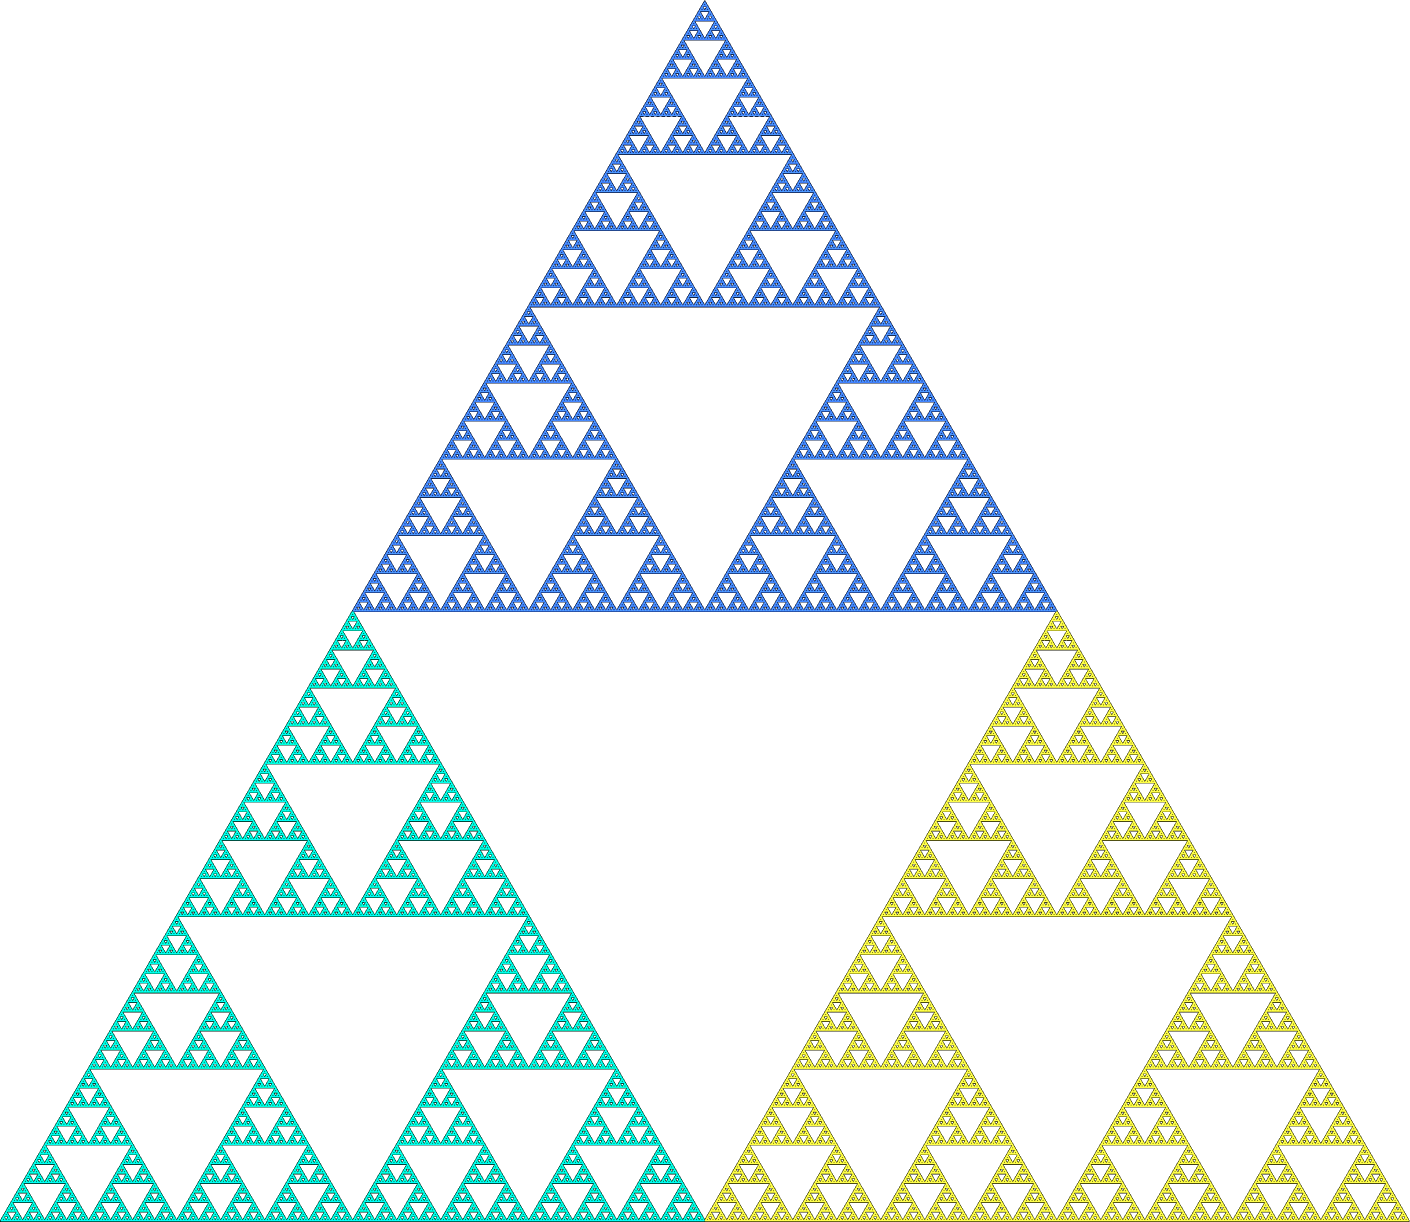
\includegraphics[width=0.3\textwidth]{SerpTri.png}
\hfill
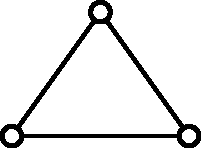
\includegraphics[width=0.3\textwidth]{SIG.pdf}
\caption{Вполне несвязное множество (слева), треугольник Серпинского и его граф пересечений.}
\end{figure}


\subsection{Критическое множество и самоподобная граница}

Пусть $\eC:=\{x:\; x\in S_i(K)\cap S_j(K),\; i,j \in I, i\neq j\}$ ---  объединение всех попарных пересечений $S_i(K)\cap S_j(K)$ (при $i\neq j$) копий первого порядка самоподобного множества $K$.
Назовём такое $\eC$ {\em критическим множеством}.
Каждая точка критического множества имеет как минимум два адреса в индексном пространстве.

Множество $\dd K:=\{x\in K: \text{ для некоторого }\bj\in I^* \text{ верно } S_\bj(x)\in \eC\}$ назовём {\em самоподобной границей} для $K$.
Говоря иначе, самоподобная граница $\dd K$ --- это множество всех предшественников точек из критического множества $\eC$.

Для любой копии $S_\bj(K)$ (при $\bj\in I^*$) мы можем найти множество её граничных точек $\dd K_\bj=\{K_\bj\cap\bigcup\limits_{\bi}K_\bi\ :\ \bi\in I^*,\ \bi\text{ и }\bj\text{ несравнимы}\}$, по которым копия $K_\bj$ пересекается со всеми остальными копиями $K_\bi$ (при несравнимых мультииндексах $\bi$ и $\bj$).
Прообраз $S_\bj^{-1}(\dd K_\bj)$ этого множества граничных точек  содержится в самоподобной границе $\dd K$.

Вообще, для любых несравнимых  $\bi,\bj\in I^*$ точка $x\in K_\bi\cap K_\bj$ является образом некоторых точек $x',x''\in\dd K$ из критического множества относительно отображений $S_\bi,S_\bj$, то есть
$$x=S_\bi(x')=S_\bj(x'').$$ 

{\em Посткритическое множество} $\eP$ системы $\eS$ --- это множество всех таких адресов $\bma=\al_1\al_2\ldots\in I^{\8}$, что для некоторых $\bj\in I^*$ справедливо $S_\bj(\pi(\bma))\in\eC$. 
Это значит, что критическое множество представляет из себя множество всех адресов точек самоподобной границы.
Для посткритического множно дать эквивалентную формулировку, согласно которой $\eP= \lbrace \sigma^k(\bma) : \pi(\bma)\in\eC, k\in \mathbb{N}\rbrace$, где отображение $\sigma^k:I^{\8}\to I^{\8}$ определяется как $\sigma^k(\al_1\al_2\ldots)=\al_{k+1}\al_{k+2}\ldots$

Система $\eS$ называется {\em посткритически конечной} \cite{Kig}, если её посткритическое множество $\eP$ конечно. 
Таким образом, если система $\eS$ посткритически конечна, то она имеет конечную самоподобную границу $\dd K=\pi(\eP)$.
Обратное неверно, поскольку точка самоподобной границы может иметь бесконечное число адресов.

\begin{example}
Рассмотрим самоподобный дендрит со следующего рисунка и отметим синим цветом точки критического множества и красным самоподобную границу.
\begin{figure}[h!]
\centering
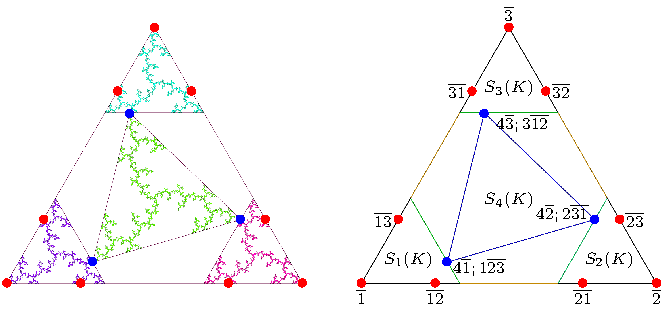
\includegraphics[width=\textwidth]{tr9.pdf}
\caption{Самоподобный дендрит, его критическое множество и самоподобная граница.}
\end{figure}
Каждая точка критического множества имеет как минимум два адреса.
В данном примере все адреса точек критического множества периодические, поэтому посткритическое множество конечно (а значит конечна и самоподобная граница).

Обозначим точки $x=\pi(4\overline{1})=\pi(1\overline{23})$, $y=\pi(4\overline{2})=\pi(2\overline{31})$ и $z=\pi(4\overline{3})=\pi(3\overline{12})$.
Самоподобную границу будут образовывать последовательности предшественников этих трёх точек по каждому адресу.
Так у точки $x$ предшественниками будут точки $\pi(\overline{1})$, $\pi(\overline{23})$ и $\pi(\overline{32}).$
У точки $y$ предшественниками будут точки $\pi(\overline{2})$, $\pi(\overline{31})$ и $\pi(\overline{13}).$
И, соответственно, у точки $z$ предшественниками будут точки $\pi(\overline{12})$, $\pi(\overline{21})$ и $\pi(\overline{3})$.
\end{example}


\subsection{Дендриты}

На протяжении всей работы особый интерес для меня будут представлять самоподобные множества, являющиеся денритами. 

\begin{restatethis}{definition}{dfn:den} %\label{dfn:den}
{\em (К. Куратовский, \cite{Kur1}; J. Charatonik, W. Charatonik, \cite{Char1998})}
{\em Дендрит} --- это локально связный континуум, не содержащий простых замкнутых дуг.     
\end{restatethis}

Простая замкнутая дуга --- это непрерывный инъективный образ окружности.
Дендриты обладают некоторыми примечательными свойствами:
\begin{enumerate}[nolistsep]
\item[1.] Любые две точки дендрита можно соединить единственной лежащей в этом дендрите жордановой дугой;
\item[2.] Любое связное подмножество дендрита само является дендритом;
\item[3.] Пересечение любых связных подмножеств дендрита связно;
%\item[4.] ...
\end{enumerate}

\begin{definition}[см. {\cite{Kur2}}]
%Если $n$ --- кардинальное число, то говорят, что пространство $X$ имеет {\em порядок} $\leq n$ в точке $p$: $$Ord(p,X)\leq n,$$ если для любого $\varepsilon>0$ существует открытое множество $G\IN X$ такое, что 
%$$p\in G,\; \diam(G)<\varepsilon\;\text{ и }\;\overline{\dd G}\leq n.$$
Если $n$ --- кардинальное число, то говорят, что пространство $X$ имеет {\em порядок} $n$ в точке $p$: $$Ord(p,X)=n,$$ если для любого $\varepsilon>0$ существует открытое множество $G\IN X$ такое, что 
$$p\in G,\; \diam(G)<\varepsilon\;\text{ и }\;\inf\{\#{\dd G}\}=n.$$
\end{definition}

Порядок $Ord(p,X)$ точки $p$ относительно дендрита $X$ называют {\em порядком ветвления}, в этом случае он совпадает с числом компонент множества $X\setminus\{p\}$.
Точки порядка $1$ в дендрите $X$ называется {\em концами} в $X$; 
точки с порядком  $2$ называется {\em разбивающими точками}; 
точки же с порядком не менее $3$ называются {\em точками ветвления} в $X$.

Континуум $X$ будет дендритом тогда и только тогда, когда $X$ локально связно и  любые две точки соединяются единственной дугой. \\

Для простого графа пересечений и критерия связности не важно, по какому множеству пересекаются копии, важен сам факт того, что пересечение непусто. 
Но в самоподобном дендрите пара копий пересекается либо по пустому, либо по связному множеству, то есть по поддендриту.
Удобнее же всего строить и изучать случаи с одноточечным пересечением.

\begin{definition}
Набор компактов $\eA=\{A_i,\ i\in I\}$ в $\mathbb{R}^n$ обладает {\em свойством одноточечного пересечения}, если для любых $i\neq j\in I$, пересечение $P_{ij}=A_i\cap A_j$ не более чем одноточечно.
\end{definition}

Мы можем определить наличие такого свойства у аттрактора системы сжимающих подобий следующим образом.
Пусть $\eS=\{S_1,\ldots ,S_m\}$ --- система сжимающих отображений в полном метрическом пространстве $X$, а $K$ --- её аттрактор. 
Пусть $\eA(\eS)=\{K_1,\ldots , K_m\}$. % и $\eA_n(\eS)=\{K_\bi:\bi\in I^n\}$.
Соответственно систему отображений $\eS$ будем называть {\em системой со свойством одноточечного пересечения}, если система $\eA(\eS)$ является системой множеств с одноточечным пересечением.

\begin{definition}
Пусть $K=K(\eS)$ --- самоподобное множество, обладающее свойством одноточечного пересечения.
{\em Граф пересечений} $\Gamma(\eS)$ системы $\eS$ --- это двудольный граф с долями $\eK=\{K_i:\; i\in I\}$ и $\eP=\{p:\;p\in K_i\cap K_j,\; i,j\in I, i\neq j\}$, и с множеством рёбер $E=\{(K_i,p):p\in K_i\}$.
\end{definition}

В графе $\Gamma(\eS)$ первой доле (белым вершинам) соответствуют копии самоподобного множества, а второй доле (чёрным вершинам) соответствуют все точки из попарных пересечений копий самоподобного множества.
Мы соединяем ребром белую и чёрную вершину, если соответствующая точка пересечения содержится в соответствующей копии.

\begin{figure}[H]
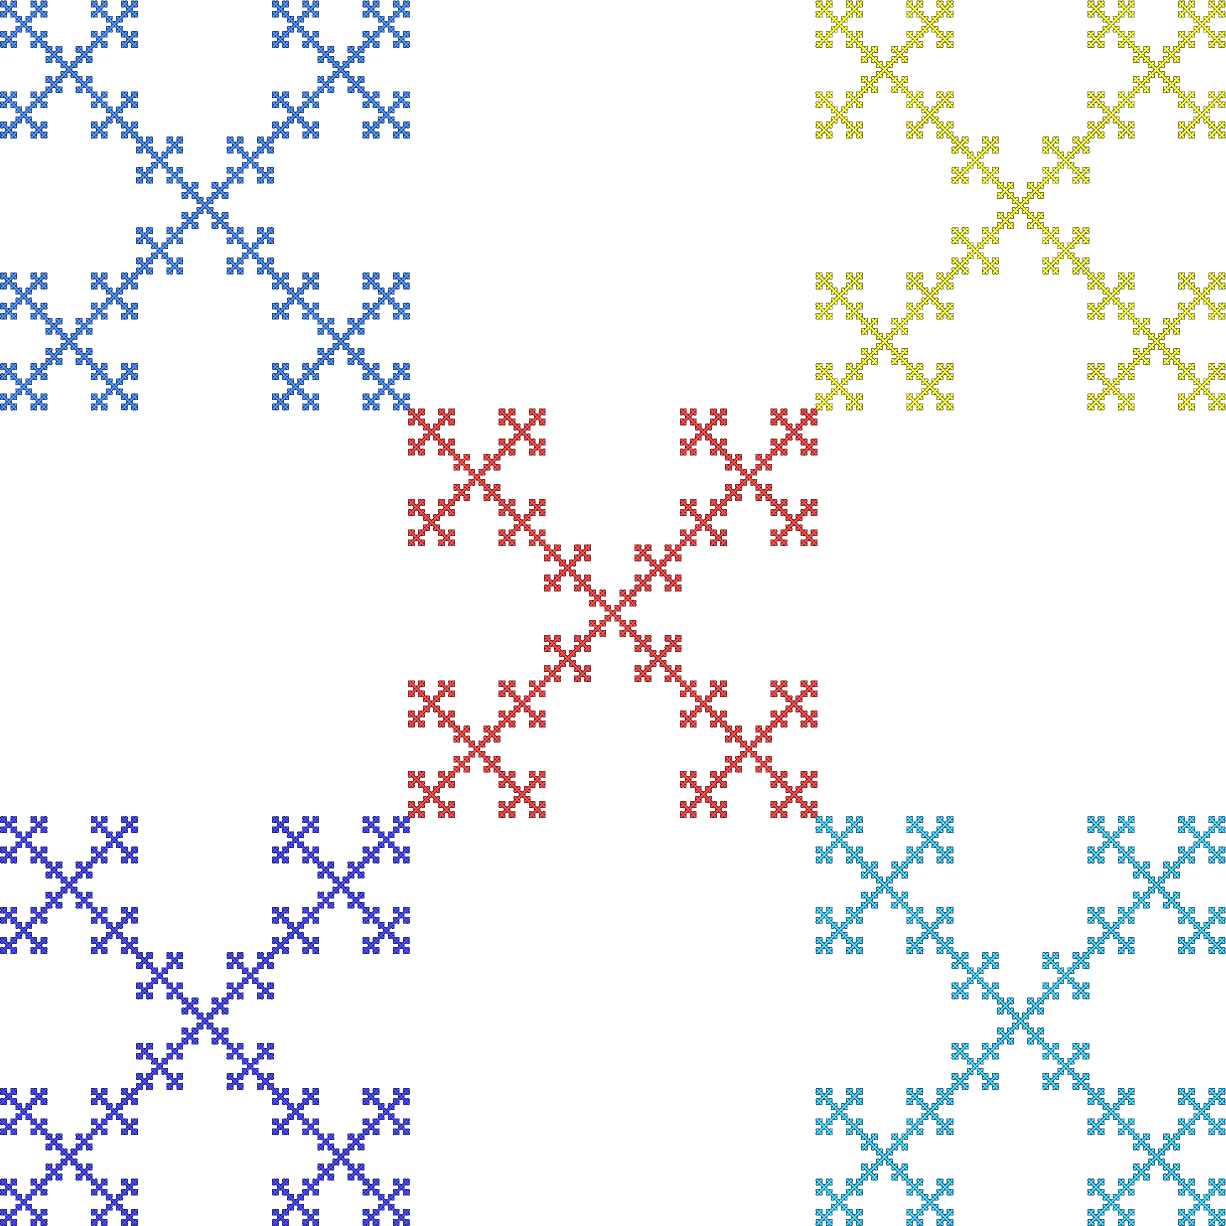
\includegraphics[width=0.4\textwidth]{VicsekSet.png}
\hfill
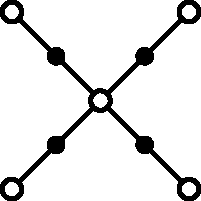
\includegraphics[width=0.4\textwidth]{BIG.pdf}
\caption{Самоподобный дендрит (слева) и его двудольный граф пересечений (справа).}
\end{figure}

Преимущество двудольного графа пересечений перед простым графом пересечений состоит в том, что тройке копий, пересекающихся по одной точке, в первом графе соответствует подграф в форме дерева, в то время как во втором графе мы получаем цикл из трёх вершин.
Это особенно полезно для следующей теоремы, позволяющей проверить, является ли самоподобное множество дендритом.

\begin{theorem}[Tetenov A. V. (2021),см. {\cite[Th.1.7]{FIP}}]
\label{thm:fpden}
Пусть $K=K(\eS)$ --- самоподобный континуум со свойством одноточечного пересечения.
Если граф пересечений $\hat\Gamma(\eS)$ системы $\eS$ является деревом, то её аттрактор $K$ --- дендрит с одноточечным пересечением.
\end{theorem}



Именно такие самоподобные дендриты с одноточечным пересечением мы и будем рассматривать во второй главе.  
И первым удобно задаваемым классом самоподобных дендритов с одноточечным пересечением являются аттракторы полигональных систем.

\section{Стягиваемые полигональные системы}

Самюэль М., Тетенов А. В. и Ваулин Д. А. в своей работе \cite{STV2017} рассматривают самоподобные дендриты, являющиеся аттракторами стягиваемых полигональных систем, которые задаются следующим образом.

%\red{Пусть также $\Om(P,A)$ обозначает угол при вершине $A$ в многоугольнике $P$.}
% используется после вторго параграфа, надо перенести туда

\begin{restatethis}{definition}{dfn:cps} \label{dfn:cps}
Пусть $P\subset\mathbb{R}^2$ --- это ограниченный многоугольник гомеоморфный диску, а $ \eV_P= \{A_1, \ldots, A_{n_P}\}$ --- множество его вершин.
Пусть дана система подобий $\eS = \{S_1, \ldots, S_m\}$ в ${\mathbb{R}}^2$ такая, что:
\begin{itemize}[nolistsep]
\item[{\bf (D1)}] для любого $i \in I$ множество $P_i = S_i (P) \subset P$; 
\item[{\bf (D2)}] для любого $i \ne j, i, j \in I, P_i \bigcap P_j =  \eV_{P_i} \bigcap  \eV_{P_j}$ и $\#(\eV_{P_i} \bigcap  \eV_{P_j})<2$;  
\item[{\bf (D3)}] $\eV_P \subset \bigcup \limits_{i \in I} S_i (\eV_P)$;
\item[{\bf (D4)}] множество $\widetilde P = \bigcup \limits_{i = 1} ^m P_i$ стягиваемо.
\end{itemize} 
Такая система  $\eS$, удовлетворяющая условиям $\bf (D1 - D4)$, называется  {\em стягиваемой $P$-полигональной системой подобий}.
\end{restatethis}

\begin{figure}[H]
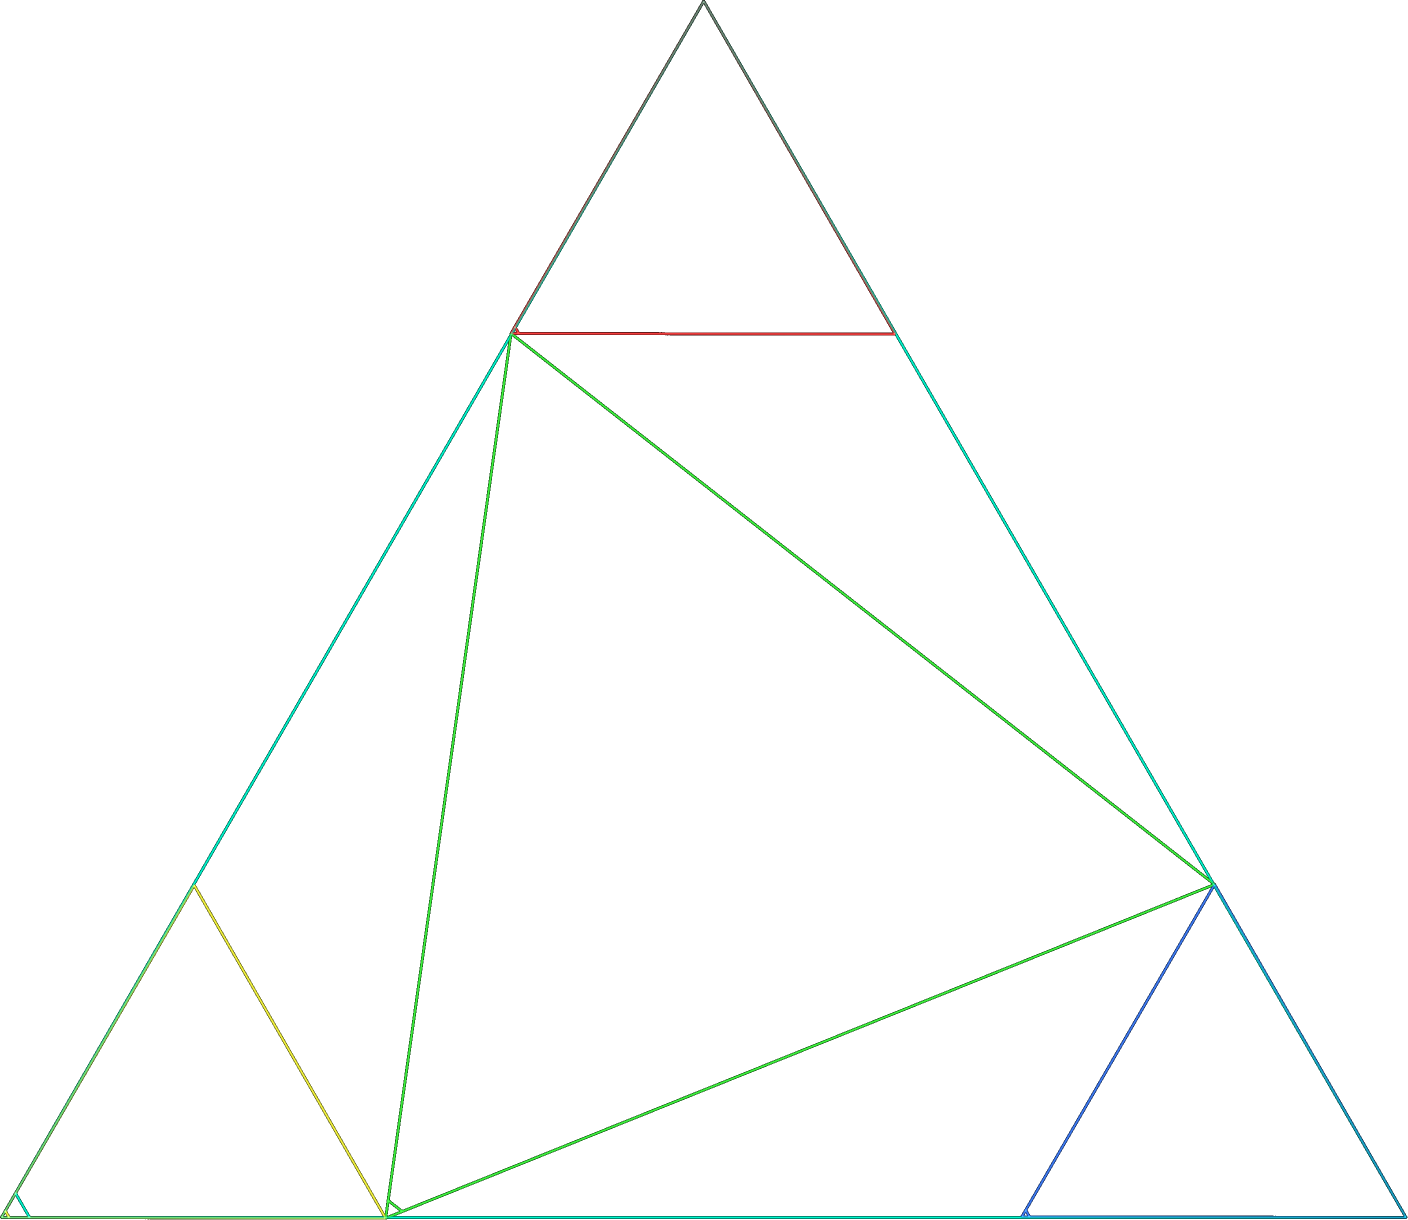
\includegraphics[width=0.45\textwidth]{CPS1_P.png}
\hfill
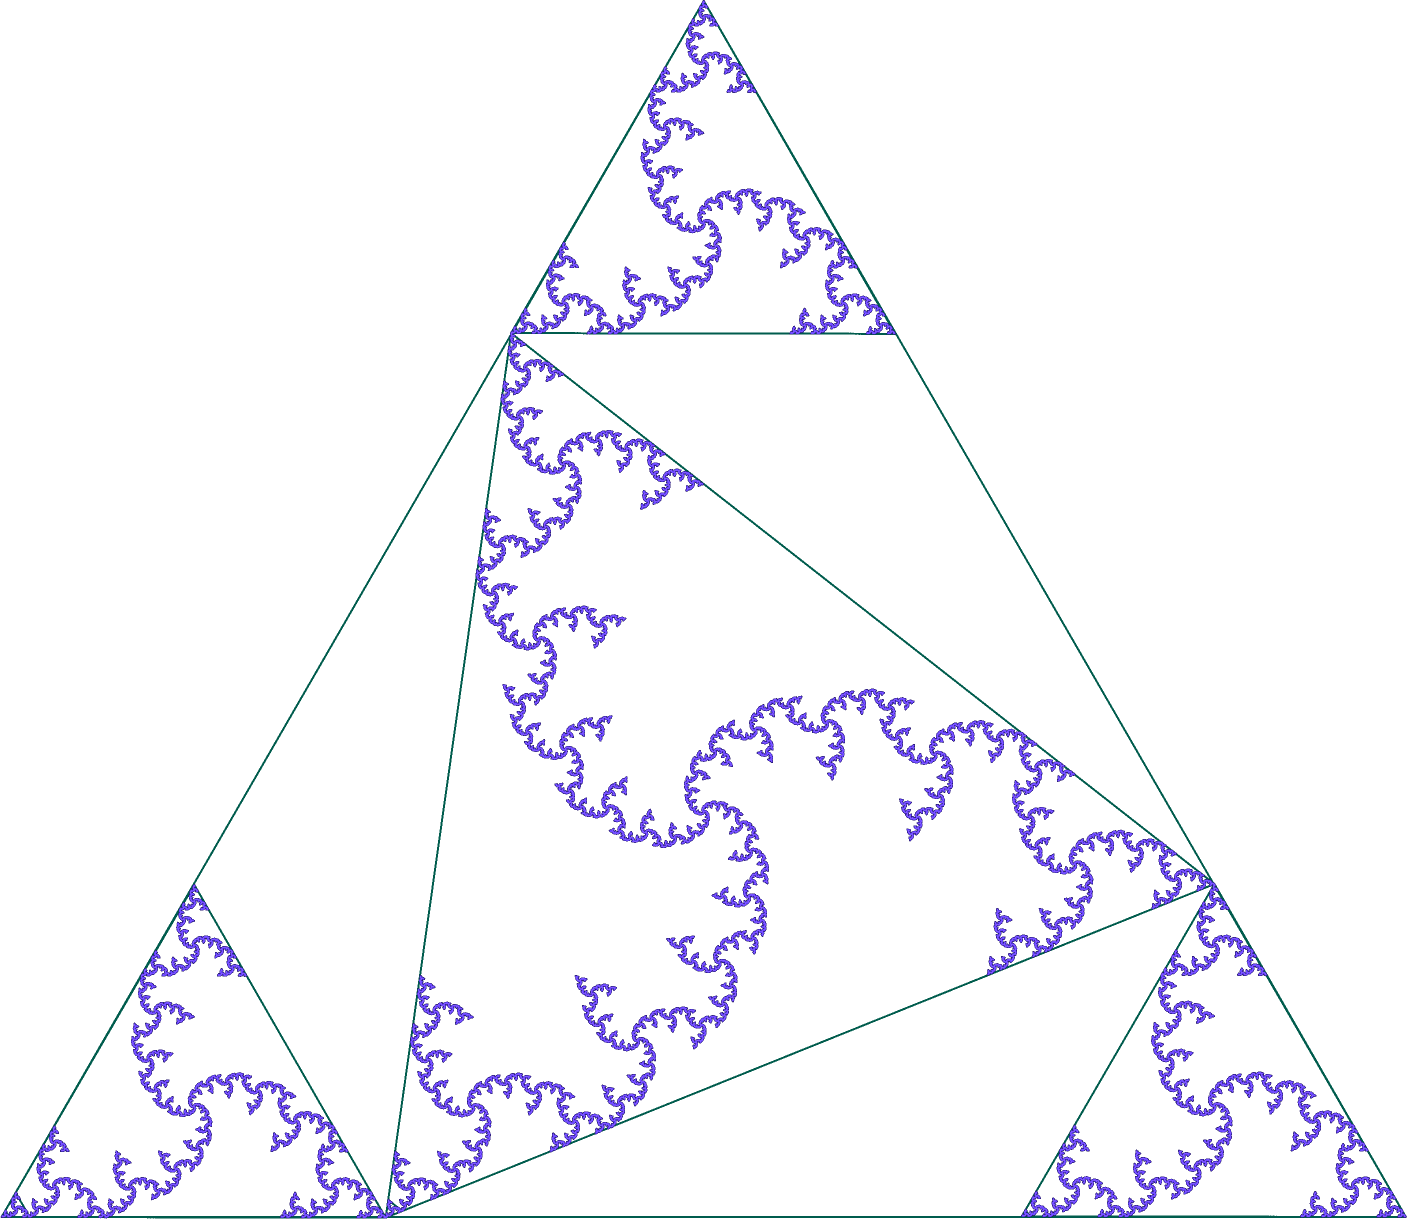
\includegraphics[width=0.45\textwidth]{CPS1_K.png}
\caption{Система многоугольников, задающая полигональную систему $\eS$ (слева), и аттрактор $K(\eS)$ этой системы (справа).}
\end{figure}

\begin{restatethis}{theorem}{thm:cpsden} %\label{thm:cpsden} 
Аттрактор $K$  стягиваемой  $P$-полигональной системы подобий $\eS$ является дендритом.
\end{restatethis}

Это действительно так, ведь из условий следует, что $K\IN P$, а значит $K_i\cap K_j=P_i\cap P_j$.
Значит, аттрактор полигональной системы --- множество с одноточечным пересечением, двудольный граф пересечения которого является деревом.
Согласно Теореме \ref{thm:fpden}, этот аттрактор является дендритом с одноточечным пересечением.\\

Авторами в \cite[Theorem 4]{TSV2017} было показано, что
\begin{enumerate}[nolistsep]
\item[1.] Всякая стягиваемая полигональная система удовлетворяет (OSC), где  в качестве открытого множества мы можем взять $\dot P$;
\item[2.] $P_\bj\IN P_\bi$ тогда и только тогда, когда  $\bj\sqsupset\bi$, а если $\bi\sqsubset\bj$, то  $ S_\bi(\eV_P)\cap P_\bj\IN S_\bj(\eV_P)$;
\item[3.] Если $\bi,\bj\in \ia$ несравнимы, то $P_\bi\cap P_\bj$ либо пусто, либо является  общей вершиной многоугольников $P_\bi$ и  $P_\bj$;
\item[4.] При этом все вершины $P$ лежат в $K$, поэтому и множество $G_\eS(\eV_P)$ вершин многогранников $P_\bj$ содержится в $K$ и плотно в $K$, а всякая точка $x\in K\mmm G_\eS(\eV_P)$ имеет единственный адрес.
\end{enumerate}
 
Во второй главе я получаю и рассматриваю обобщение таких полигональных систем.



\section{Главное дерево}

\begin{figure}[H]
\center{
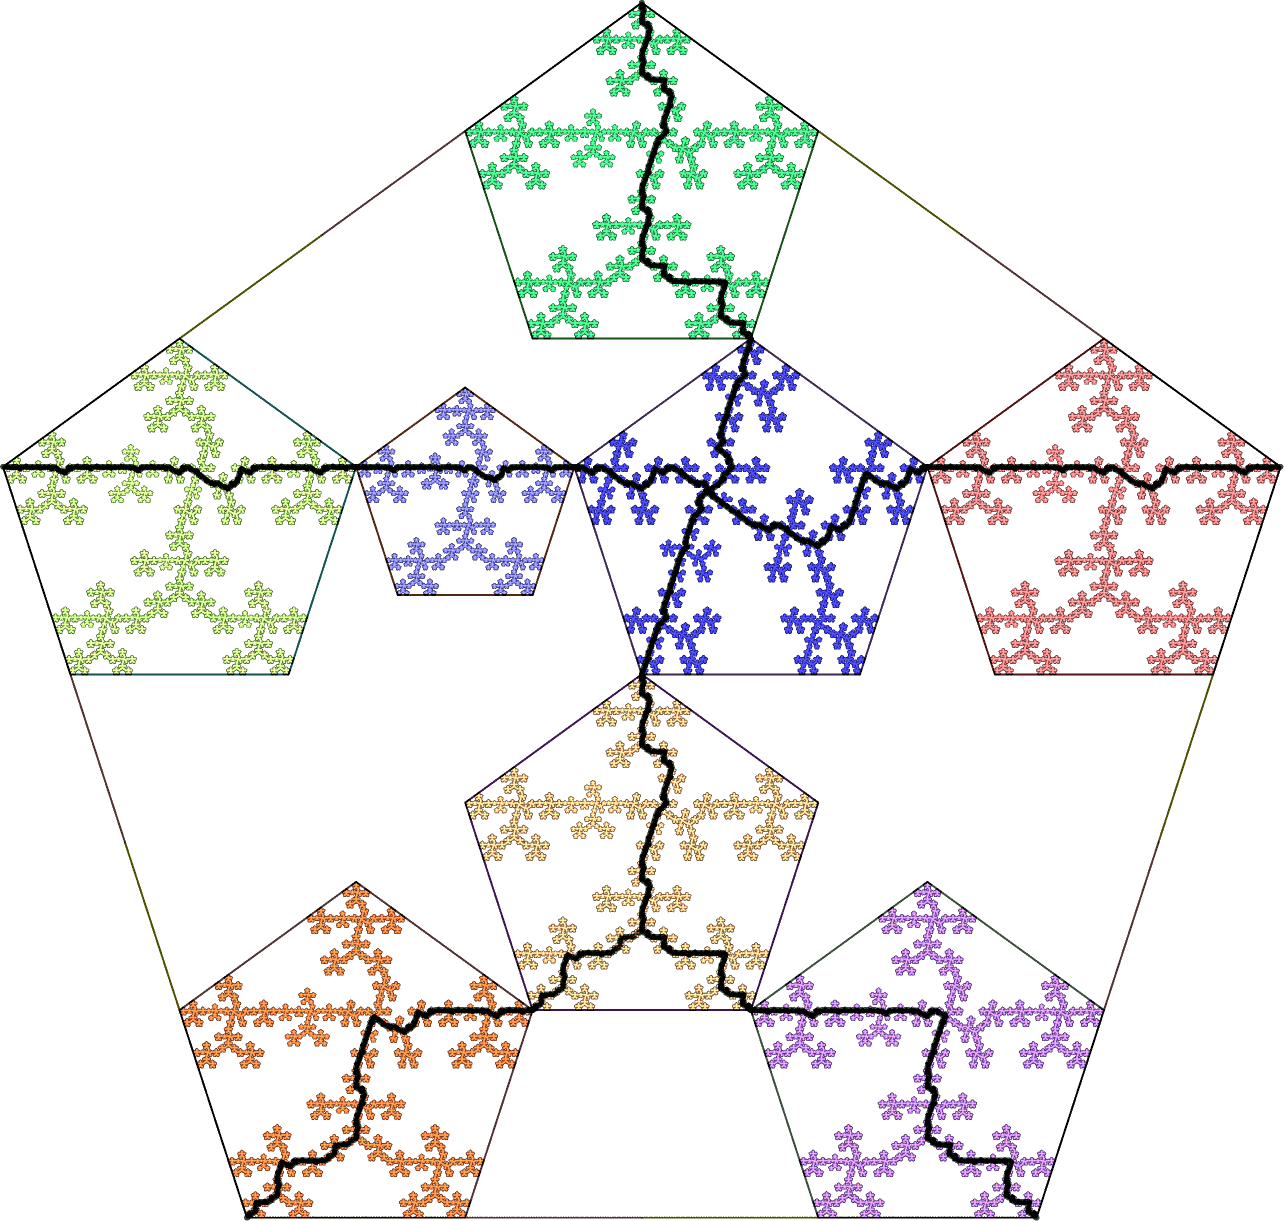
\includegraphics[width=0.5\textwidth]{penta4plus3.png}}
\caption{Полигональный дендрит $K$ c $\dd K=\eV_P$ и его главное дерево $\hat\gamma$. }
\label{fig:penta4plus3}
\end{figure}

Если $K$ --- самоподобный дендрит, то любую пару точек $a_i,a_j\in\dd K$ из его самоподобной границы можно соединить единственной жордановой дугой $\gamma(a_i,a_j)\IN K$.
Такие дуги, соединяющие пары точек самоподобной границы дендриты, мы будем называть {\em главными дугами}.
Если самоподобная граница $\dd K$ самоподобного дендрита конечна, то множество всех главных дуг тоже будет конечно.
Объединение всех главных дуг будем называть {\em главным деревом}.

\begin{definition}\label{dfn:MT}
Пусть $K$ --- самоподобный дендрит c конечной самоподобной границей $\dd K$. 
Минимальный поддендрит $\hat\gamma\IN K$, содержащий $\dd K$, называется {\em главным деревом} дендрита $K$.
\end{definition}

Главное дерево $\hat\gamma$ самоподобного дендрита $K$ с одноточечным пересечением обладает следующими очевидными свойствами:
\begin{enumerate}[nolistsep]
\item[1.] $\{x\in\hat\gamma:Ord(x,\hat\gamma)=1\}\IN\dd K$, то есть концами главного дерева могут быть только точки самоподобной границы;
\item[2.] $2\leq\#\{x\in\hat\gamma:Ord(x,\hat\gamma)=1\}\leq\#\dd K$;
\item[3.] $Ord(x,\hat\gamma)\leq Ord(x,K)$;
\item[4.] .
\end{enumerate}

На рисунке \ref{fig:penta4plus3} показаны аттрактор полигональной системы и его главное дерево. 
В этой системе самоподобной границей будут вершины большого пятиугольника.
Разумеется, концами главного дерева могут быть только точки самоподобной границы.
В этом конкретном примере каждая точка самоподобной границы является концом в главном дереве, но вообще эти точки могут быть и разбивающими.
Тем не менее, в главном дереве не может быть меньше двух концов.

%%%%%%%%%%%%%%%%%%%%%%%%%%%%%%%%%%%%%%%%%%%%%%%